\documentclass[10pt,twoside]{article}
\usepackage{graphicx}
\usepackage{wrapfig}
\begin{document}

\title{The Cellophane sheet visualization}
\date{Complied with \LaTeX{} on \today}
\maketitle
\begin{center}
{\scriptsize Copyright (c) 2007 Ramkumar Ramachandra,
artagnon@gmail.com\\ Permission is granted to copy, distribute and/or
modify this document under the terms of the GNU Free Documentation
License, Version 1.2 or any later version published by the Free
Software Foundation; with no Invariant Sections, no Front-Cover Texts,
and no Back-Cover Texts.}
\end{center}

\subsection*{Disclaimer}
This paper contains original unverified research. The author is not responsible
for any damages caused to intellectual property by reading, sharing or
distibuting this paper, both legally and illegally. Use at your own risk!

\subsection*{Preface}

\begin{wrapfigure}{r}{20mm}
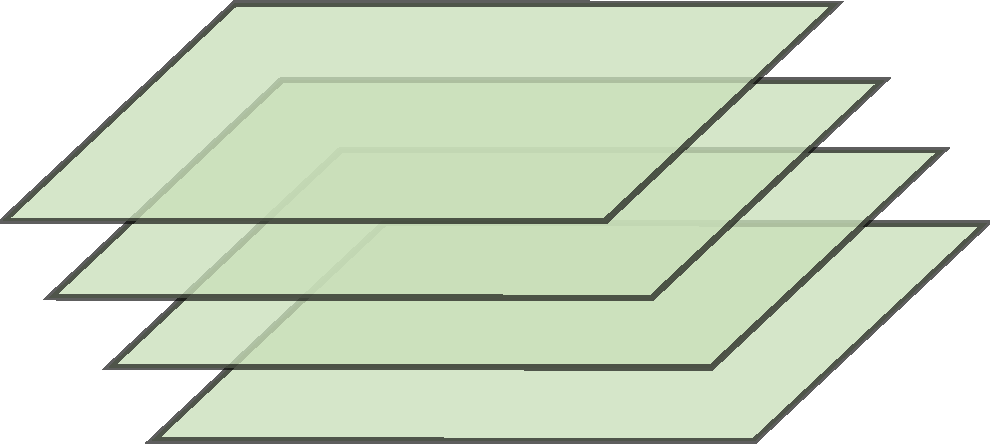
\includegraphics[width=20mm]{res/logo.pdf}
\end{wrapfigure}

The objective of this paper is to make life with pointers easier. This article
applies mainly to C and C++ but the syntax can be extended to just about any
programming language which uses the kind of pointers that C/ C++ uses. The
cellophane sheet technique is a powerful technique of visualising and evaluting
complicated expressions like \&(**(*a+5)+6) easily. Although such applications
may be attributed to academic importance, this technique was created primarily
to help the beginner grasp the concept of pointers.


\subsection*{What is a variable?}
All memory locations can be, for the purpose of illustration, broken up into two
parts: The address part which contains the address of the memory location and
the data part which contains the data stored in that memory
location.\footnote{In reality, address isn't ``stored'' in the memory location.
Address is just the inherent property of every memory location} When a
``variable'' is declared, it means that the compiler simply gives the user the
convinience of naming the memory location with a name. For example, in the
statement ``int a'' picks a suitable random memory location from the memory of
the computer and names it ``a'' for the purpose of convinience of the
programmer.  \newpage \subsection*{What then, is a pointer?}

\begin{wrapfigure}{r}{55mm}
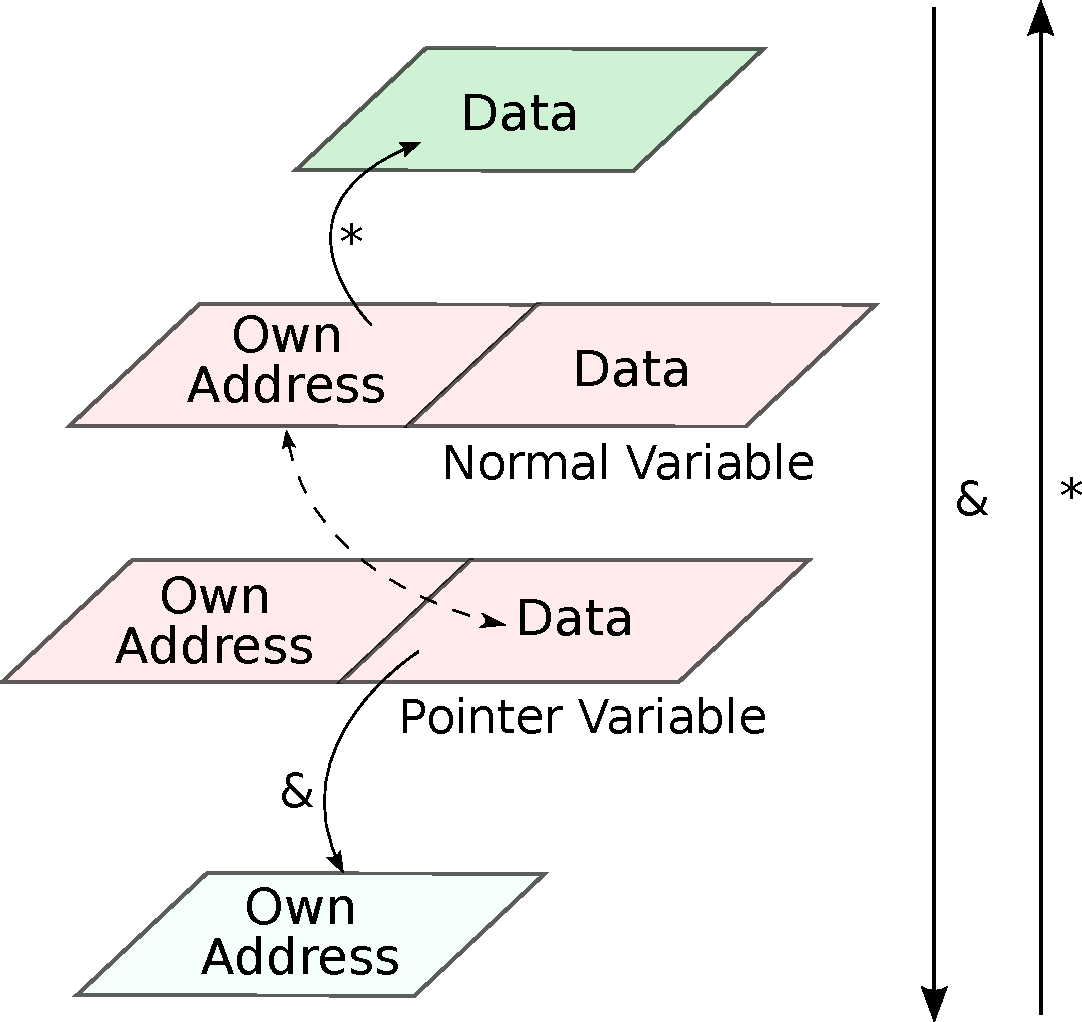
\includegraphics[width=55mm]{res/variable-pointer.pdf}
\end{wrapfigure}

A pointer, or a pointer variable is also a variable. It behaves almost exactly
like a normal variable. The only difference is that when an integer variable
stores a number like 97 in its data part, a pointer variable stores a number
like 7eb012c3\footnote{On a 32-bit system} which refers to the address of
another ``variable''. Attempting to print a variable prints its data part. Using
the (\&) operator on a variable returns its address part. Using the (*) operator
on a variable finds another variable with the address mentioned in the data part
of the variable.  It returns the data part of the variable found. For example,
in ``int *a, b; a = \&b;'', the data part of \textit{a} contains the address of
\textit{b}. Therefore *a would first find b and then return b's data part. In
this example, we could say that \textit{a} is ``pointing to'' \textit{b}.
\subsection*{Variable types} Every variable type has two portions in the
specification: The data type and the ``pointer level''.\footnote{Pointer level
is a term coined by the author for the purpose of explanation only} The pointer
level indicates how many times the (*) operator needs to be used in order to get
to the real data and not just another address. For example, ``int **a'' makes
variable \textit{a} of data type int and pointer level 2 (or simply int**). It
is hence a ``pointer to a pointer''. This means that a is pointing to the
variable *a, which in turn is again pointing to **a. The data part of **a
contains the real data.

In the case of variables of pointer level 0 or ``normal variables'', the data
type indicates how many bytes of memory are required to store the variable's
data and how the data's variable is stored.

In the case of variables of pointer level {\textgreater}=1, the memory allocated
and the method of storing the address is constant. The data type simply
indicates the data type of the variables pointed to by the pointer. ``float *a''
for example makes variable \textit{a }\textup{a pointer of level 1 and data type
float. This means that it is ``pointing to'' a float variable of level 0. Note
again that in both ``float *a'' and ``int *b'', }\textit{a}\textup{ and
}\textit{b }\textup{are of the same size.} \newpage \subsection*{Familiarization
with the notation}

\begin{wrapfigure}{r}{70mm}
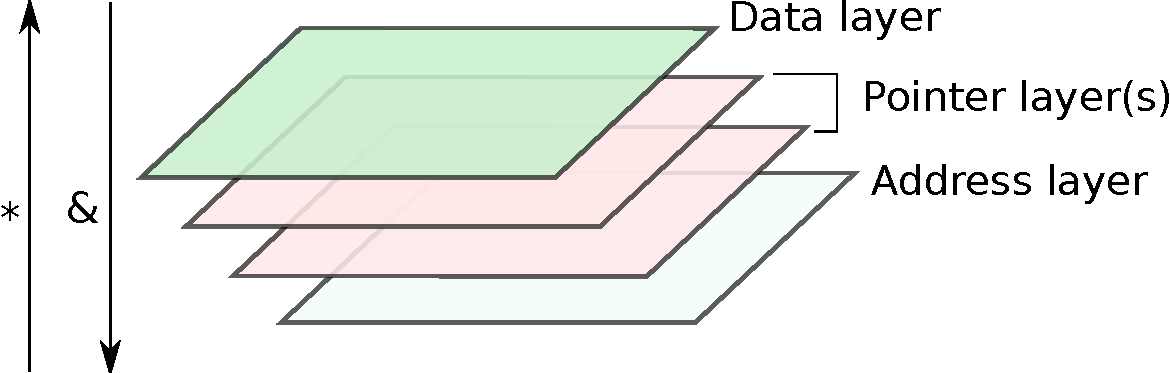
\includegraphics[width=70mm]{res/layer-splitup.pdf}
\end{wrapfigure}

The whole memory can be visualized as a set of layers. There are a minimum of
two layers: the data layer and the address layer. As we add levels of pointers,
the number of layers increase. The (\&) operator enables one to move down layers
and the (*) operator enables them to move up layers. Each of these layers is
made of thin transparent cellophane sheets so one can look through the layers.

\begin{wrapfigure}{r}{70mm}
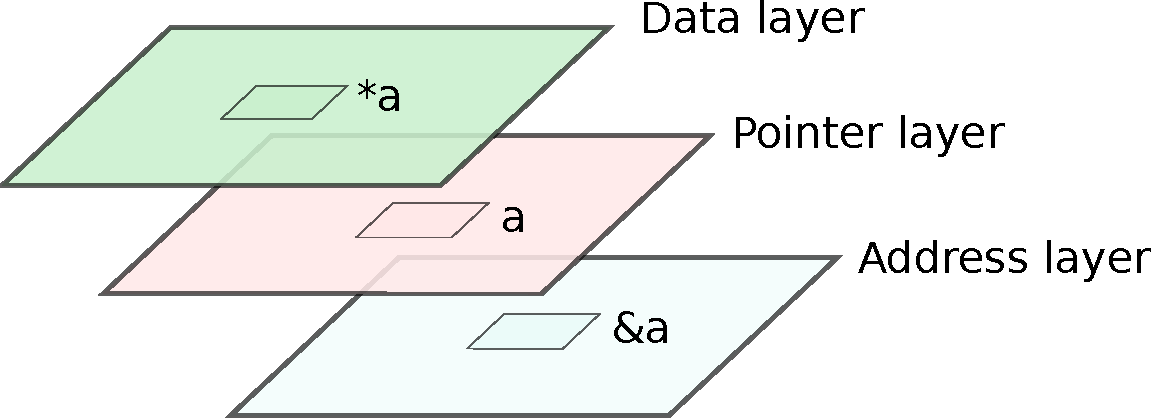
\includegraphics[width=70mm]{res/simple-pointer.pdf}
\end{wrapfigure}

A simple pointer (declared using int *a) has been represented in the cellophane
sheet layer notation in the figure on the right. There is only one pointer layer
as \textit{a} is a pointer variable.

\subsection*{Examples and exercises}
\subsubsection*{Example}

\begin{wrapfigure}{r}{70mm}
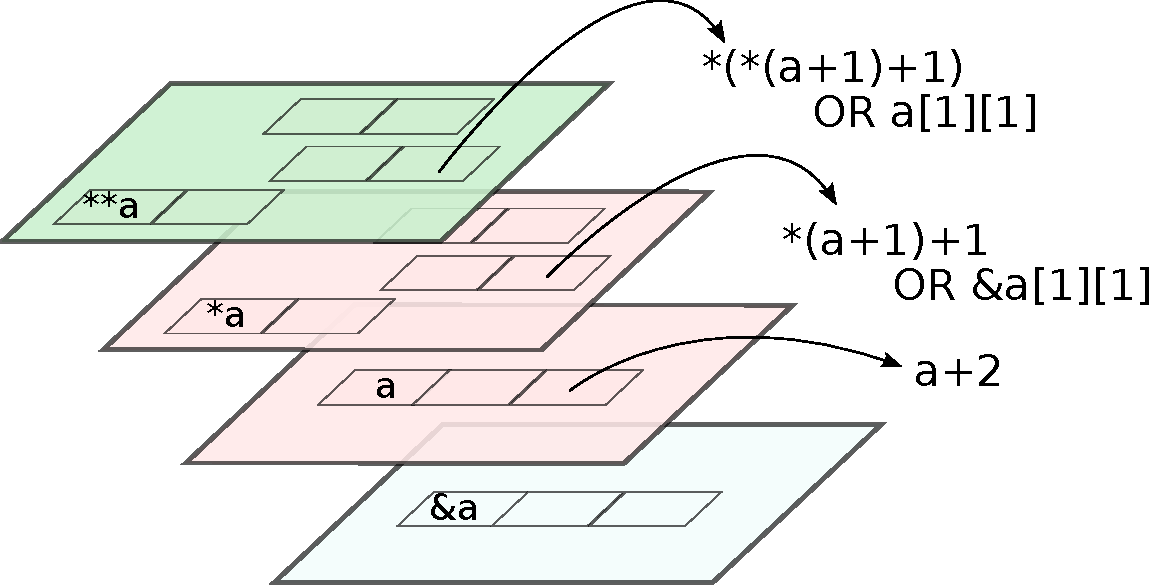
\includegraphics[width=70mm]{res/dual-ar.pdf}
\end{wrapfigure}

Consider the declaration int a[3][2]. Clearly, \textit{a }\textup{is of type
int**. For the visualization, the number of layers equals 2+(highest pointer
level) = 2+2 = 4. The lowest layer is the address layer, the highest is the data
layer and there are two intermediate pointer levels which refer to a, *a and
their neighbours.  First analyse what the declaration does. It creates three
consecutive memory locations in the second layer, three sets of two consecutive
memory locations in the third layer. We now create the data and address layers
as shown. Think of the model as a tree where the base three branches branch off
to two sub-branches each. The rest of the information can be deduced from the
diagram as shown.}

\subsubsection*{Exercises}
Visualize: \&(*a), *(\&a), ***a, \&(**(*a+5)+6), **(a[1]+1),
*a[0][1]+1+4
\newpage
\end{document}
